% The proposed method {\em someMETHOD}
% has the following advantages:
% \bit
% \item it gives better classification accuracy than all 10 competitors we tried
% \item its accuracy is very close to the very best competitor
%       in the {\em UCR Insect Classification Contest}.
% \item it is scalable
% \eit



\subsection{Preliminary Result (Phase 2)}

We ran our implemented D-Cube algorithm on the Darpa TCP Dump datasets. Also, we bucketize all timestamps by hour. The following tables present several statistics and properties on the found dense blocks, as well as global features like elasped run time. 
Further experiments and analysis will be carried out in the final phase of our project. Today, we just simply present the statistics for a bird view of the big picture. \\
We ran the D-Cube algorithm to find five dense blocks using $k = 5$ and tested different combinations of methods/metrics. The results are shown in Table \ref{tbl:stat}.\\ 

\textbf{Abbreviation}
\bit
\setlength\itemsep{0.8em}
\item \textbf{Ari:} "Arithmetic Average Mass" 
\item \textbf{Geo:} "Geometric Average Mass" 
\item \textbf{Susp:} "Suspiciousness"
\eit

\subsection{Final conclusions}

We have implemented D-Cube, an effective algorithm to detect and extract dense blocks in multi-aspect data, to perform anomaly detection. Applications can vary from detecting network attaks among TCP/IP connections, identifying paid or malicious reviewers in Amazon or Yelp, etc. We performed multiple experiments on different datasets and report the statistics on the detected dense blocks, moreover, we also gave explanation and justification on whether the retrieved records in the dense blocks are interesting anomalies. To conclude, D-Cube algorithm successfully perform the tasks and the results match our expectation. What's more, D-Cube is a disk-based algorithm that can extensively handle gigantic data that are too large to fit in memory. 

\begin{table}[h!tbp] 
  \caption{Overall Statistics of Dense Blocks}\label{tbl:stat}
  \begin{tabular} {p{1.5cm}|p{2cm}|p{12cm}}
    \hline \parbox[t]{1.5cm}{Density\\Measure} & \parbox[t]{2cm}{Dimension\\Selection} & Results \\
      \hline Ari & Cardinality & \parbox[c]{1em}{
      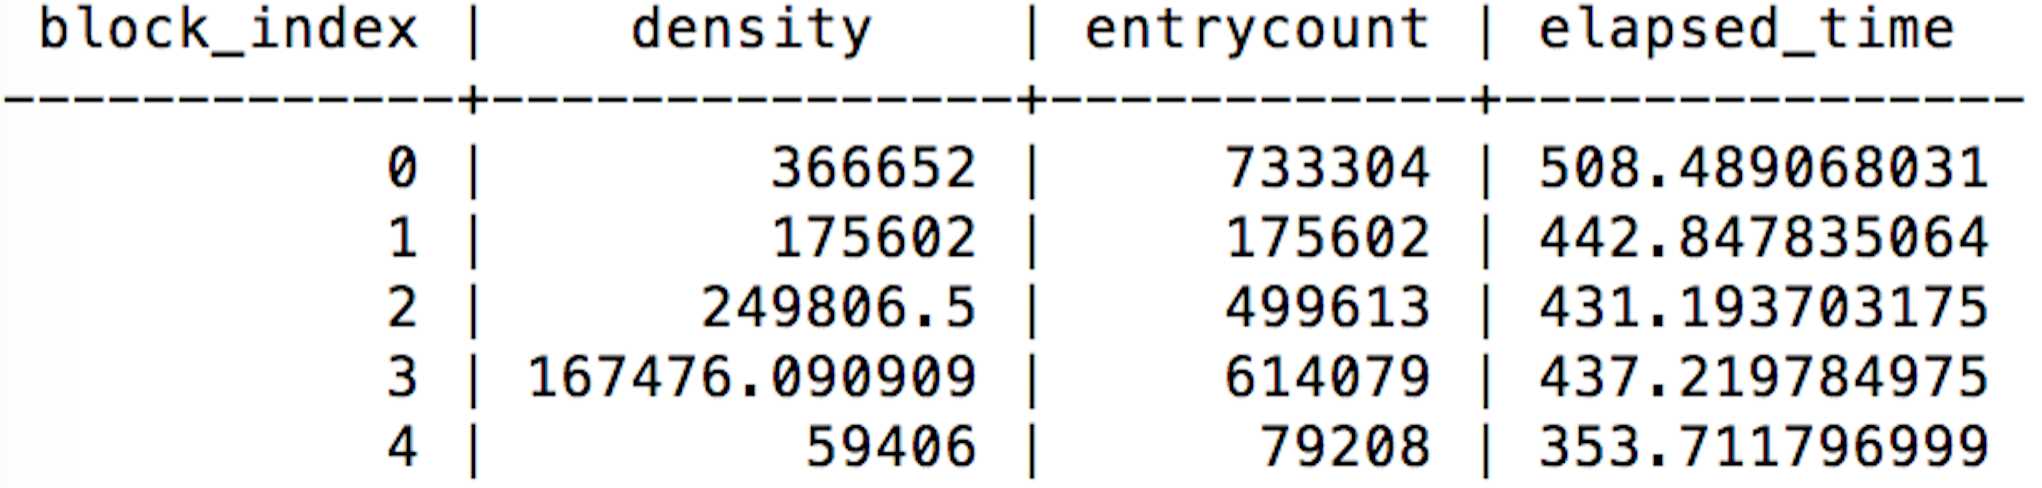
\includegraphics[width=5in]{report_table_arith_car.png}} \\
      \hline Ari & Density & \parbox[c]{1em}{
      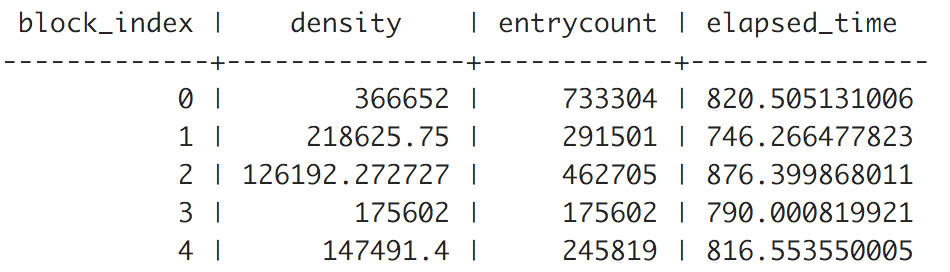
\includegraphics[width=5in]{report_table_arith_density.png}} \\
      \hline Geo & Cardinality & \parbox[c]{1em}{
      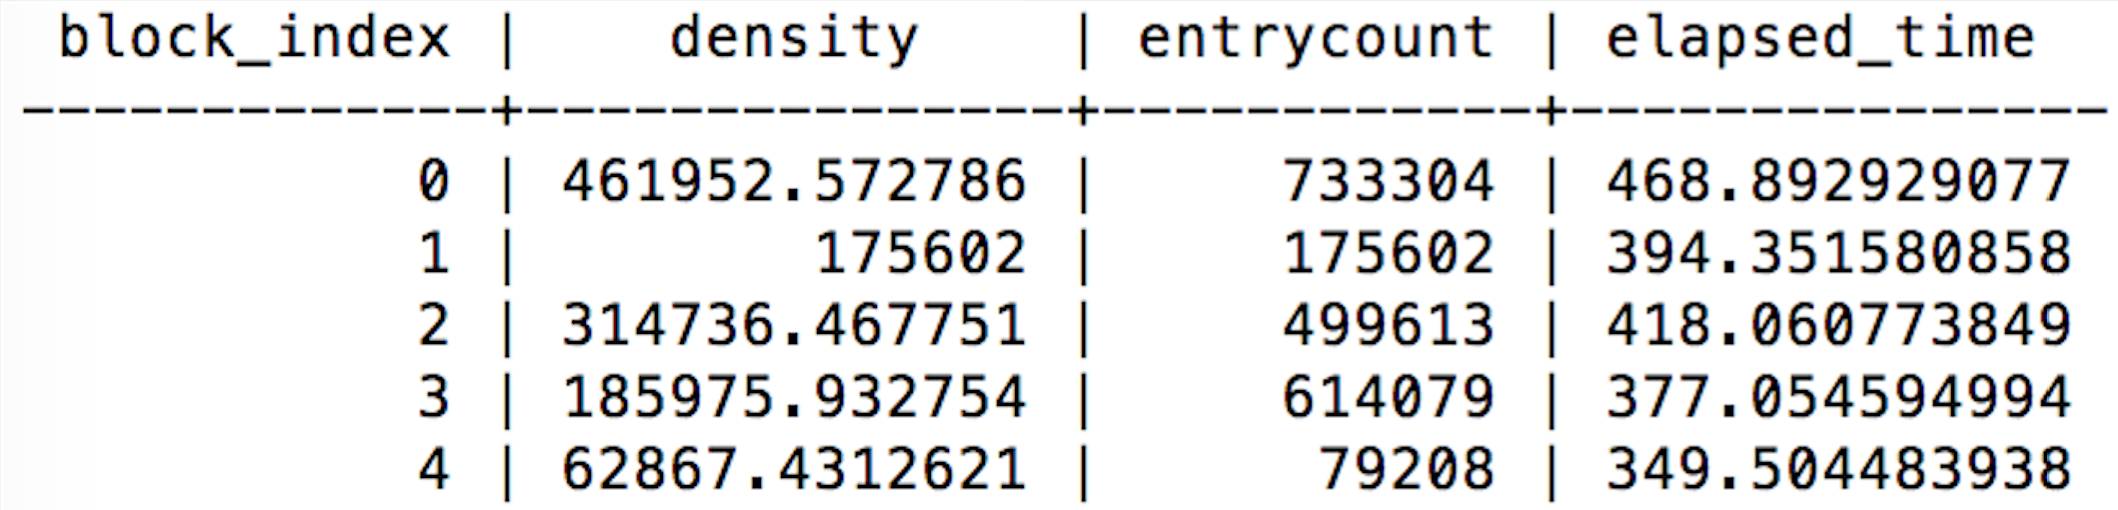
\includegraphics[width=5in]{report_table_geo_car.png}} \\
      \hline Geo & Density & \parbox[c]{1em}{
      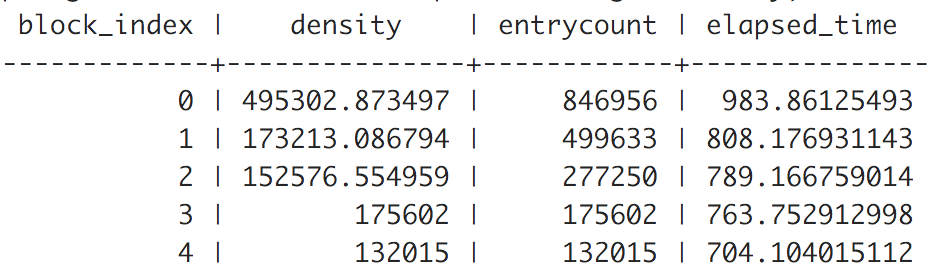
\includegraphics[width=5in]{report_table_geo_density.png}} \\
      \hline Susp & Cardinality & \parbox[c]{1em}{
      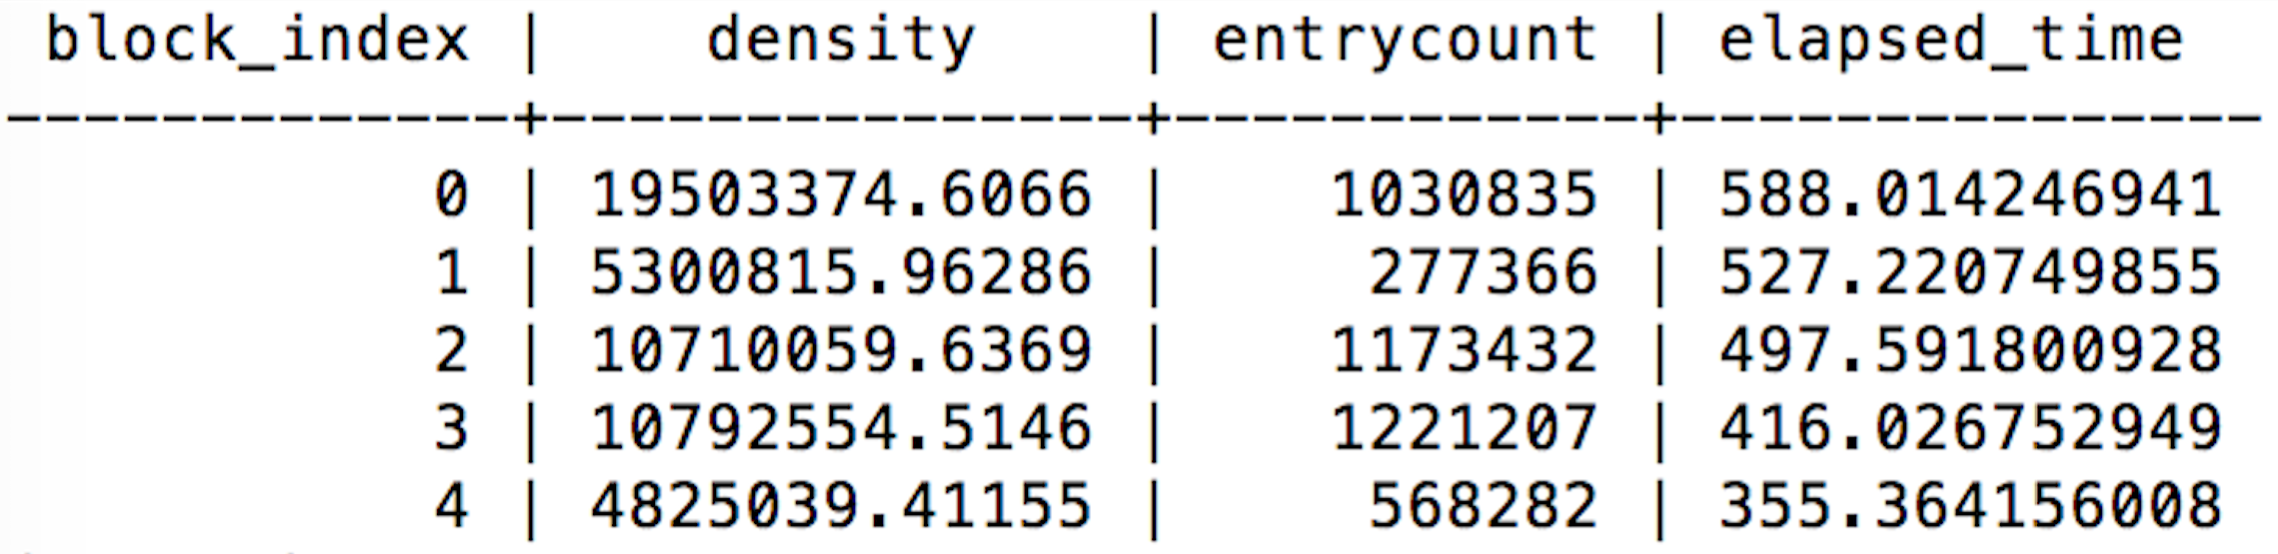
\includegraphics[width=5in]{report_table_sus_car.png}} \\
      \hline Susp & Density & \parbox[c]{1em}{
      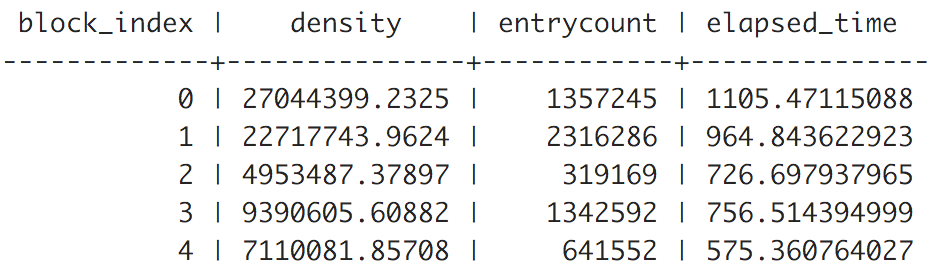
\includegraphics[width=5in]{report_table_sus_density.png}} \\
      \hline
  \end{tabular}
\end{table}


